% !TEX encoding = UTF-8
% !TEX TS-program = pdflatex
% !TEX root = ../nt.tex
% !TEX spellcheck = it-IT

%************************************************
\chapter{DATA WAREHOUSE}
\label{cap:dw}
%************************************************\\


\section{Introduzione}

Finora abbiamo parlato dei database relazionali. I data warehouse non sono database fatti per il 
CRUD, ma sono adatti soprattutto per il calcolo o l’analisi dati (letteralmente data warehouse 
significa magazzino di dati) e differiscono dai database perché possono essere visti come una sorta 
di database di database. 

Esistono dei prodotti software per costruire data warehouse; nel mondo open source abbiamo: 

\begin{itemize}
\item Pentaho 
\end{itemize}

Invece nel mondo del business abbiamo delle estensioni che permettono di gestire il 
multidimensionale, quali: 

\begin{itemize}
\item Oracle;
\item Analisys Services (un’estensione di Microsoft SQL Server). 

\end{itemize}

Per certi versi il mondo dei data warehouse somiglia al mondo dei database relazionali: anche qui useremo la modellazione a tre livelli (concettuale, logica e fisica), tuttavia il mondo dei database analitici è diverso per altre ragioni.

\begin{center}
\begin{figure}[H]
\centering
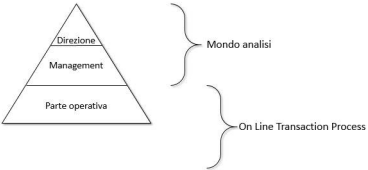
\includegraphics[scale=1]{figures/dmo2.png}
\caption{Piramide DMO di Anthony}
\end{figure}
\end{center}

Alla base della piramide di Anthony vi è il livello del transazionale (On Line Transaction Processing) che può essere visto come un’operazione CRUD o un insieme di relazioni CRUD interpretate come un unico oggetto. Questo è il mondo delle transazioni, diverso da quello dell’analisi. Cominceremo a prendere dimestichezza con l’ambito dei data warehouse quando avremo a che fare non tanto con gli aspetti operativi delle aziende, quanto piuttosto con quelli manageriali o dirigenziali. Questi progetti sono molto costosi: a differenza di quelli transazionali che vanno da mille a un milione di euro, quelli di data warehouse hanno un costo da alcune decine di milioni di euro in su. Un progetto può arrivare a costare tanto poiché richiede lo sforzo di creare il contesto lavorativo giusto nel quale far funzionare l’informatica.  

In genere nella pubblica amministrazione si dispone delle informazioni, si aggregano, sintetizzano e le si inviano ai piani superiori. Questo insieme di operazioni hanno dei “Key Performance Indicator” e sono dei dati sintetici rivolti ai dirigenti. Solitamente nella pubblica amministrazione le idee su cosa debba essere un indicatore sono poche, confuse e gestite male. Calcolare un indicatore è sempre qualcosa molto meno banale di quello che sembra: generalmente abbiamo indicatori molto sofisticati e capirne il significato e le implicazioni è molto complicato. 


\section{Analisi multidimensionale}

La teoria che c’è dietro il data warehouse è di natura geometrica: parliamo di analisi 
multidimensionale, pattern recognition (i.e., concetto di causalità e correlazione o effetto), Business Intelligence e machine learning. 

Possiamo fare una proiezione per rappresentare un cubo su un piano, quindi avremo l’immagine 2D di un oggetto 3D. Uno spazio di dimensione n può contenere solo oggetti di dimensione $\leq n$. Il problema delle proiezioni è la perdita di informazioni, d’altra parte permette di continuare a rappresentare almeno una vista di un oggetto a n dimensioni su uno spazio a $k$ dimensioni con $n > k$. Se non volessimo perdere informazioni, dovremmo rappresentare tutte le viste (cioè un numero minimo che ci consenta di avere tutte le informazioni): così facendo potremmo ricostruirlo esattamente. 

\begin{center}
\begin{figure}[H]
\centering
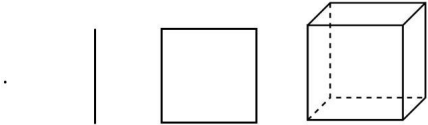
\includegraphics[scale=1]{figures/dimensions.png}
\caption{Varie dimensioni}
\end{figure}
\end{center}

Chiarito il concetto di proiezione, possiamo anche fare proiezioni di ordine superiori, ad esempio un ipercubo sul piano della lavagna. Per farlo cominciamo a disegnare il cubo di partenza e poi, sapendo dalla fisica che lo spazio tempo è in 4 dimensioni, lo replicheremo tante volte quante ne occorrono per rappresentare la sua traiettoria. Rappresento quindi il cubo e tutte le sue posizioni temporali al tempo $t$.

\begin{center}
\begin{figure}[H]
\centering
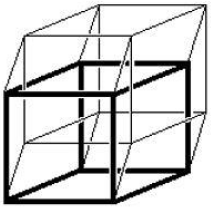
\includegraphics[scale=1]{figures/hc1.png}
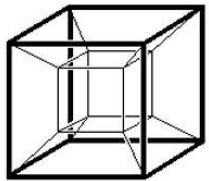
\includegraphics[scale=1]{figures/hc2.png}
\caption{Ipercubi multidimensionali}
\end{figure}
\end{center}

Allo stesso modo possiamo disegnare un ipercubo disegnando delle diagonali che si allontanano dai vertici del cubo: consideriamo uno spigolo solido e tracciamone un 
altro che si allontana dal centro dell’oggetto: replicando questa operazione per tutti gli spigoli, otterremo un cubo che si gonfia. Bisogna immaginarlo come un oggetto solido 
a 4 dimensioni pensando a n repliche del cubo di dimensione $\{x,\ x+\delta,\ x+2\delta\}$ e così via: lo spazio intermedio è pieno con una densità a 4 dimensioni, ci sono 
più copie del cubo contemporaneamente nello stesso posto.

A questo punto possiamo astrarre il concetto di rappresentazione di un punto geometrico e riferirlo non più allo spazio dei punti ma a quello dei dati. Ad esempio immaginiamo il solito database cliente-acquista-prodotto. Cosa significa dire cliente? Significa considerare uno spazio lineare di clienti dove i punti potenzialmente possono assumere qualsiasi valore possibile. Quindi immaginare uno spazio lineare in cui ordinare secondo un certo criterio i clienti significa rapportare un tipo di entità a uno 
spazio lineare su cui vale una relazione d’ordine definita tramite l’id. Ogni id identifica univocamente un cliente ed è un oggetto definito su uno spazio lineare dei numeri interi.

\begin{center}
\begin{figure}[H]
\centering
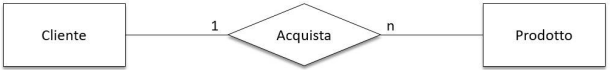
\includegraphics[scale=0.8]{figures/cap3.png}
\caption{Cliente Acquista Prodotto}
\end{figure}
\end{center}

Cosa significa dire cliente-acquista-prodotto? Se abbiamo lo spazio dei clienti e lo spazio dei prodotti, la relazione è una coppia cliente-prodotto: avremo quindi un punto all’interno di uno spazio ad n dimensioni che rappresenta i fatti di interesse del database. Così abbiamo trasformato la teoria dei diagrammi entità-relazione in una teoria di geometria sugli spazi astratti dei dati. Questa è la \underline{teoria multidimensionale dei dati}. È interessante perché riusciamo a trasformare operazioni di analisi sui dati in operazioni di analisi sulle figure. Il problema è che in un database dove ci sono 10 tipi di entità dobbiamo lavorare in uno spazio a 10 dimensioni e inoltre, se ci sono tante relazioni, 
non basterà un punto per rappresentare un fatto, ma molti tipi diversi di punti che legano queste dimensioni. Quando combiniamo i punti attraverso i tipi di relazione otteniamo delle n-ple che rappresentano i fatti di interesse all’interno dello spazio multidimensionale.  

$\rightarrow$ Fare una query su database significa estrarre un oggetto da uno spazio a n dimensioni. 

Consideriamo ora la relazione prodotto-negozio-data (relazione ternaria di vendita) in uno spazio a n dimensioni. Questi oggetti non sono dei tipi di entità, per il momento possiamo chiamarli database. In tal modo abbiamo un database con tutti i prodotti, uno con tutti i negozi e uno dove ci sono tutte le date in cui è stata effettuata una vendita.  

\begin{center}
\begin{figure}[H]
\centering
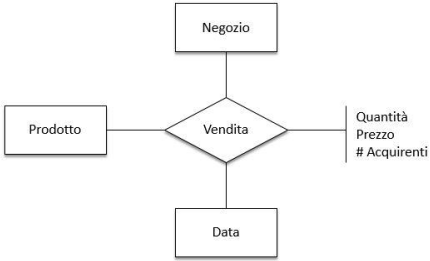
\includegraphics[scale=1]{figures/vendita.png}
\caption{Vendita FACT}
\end{figure}
\end{center}

All’interno di questo spazio consideriamo un cubo, questo rappresenta una data di inizio e una di fine, un prodotto di inizio e uno di fine, poi un negozio di inizio e uno di fine. Fare le query sul database significa tagliare a fette e poi a cubetti (slice and dice) il cubo di origine, dove ogni cubetto rappresenta un fatto elementare o un’istanza di questa relazione. Per ogni fatto andiamo a rappresentare sul diagramma entità relazione la quantità, il prezzo, il numero degli acquirenti (dato che il database è analitico e dobbiamo fare l’operazione di aggregazione ci serve contare gli utenti per n transazioni andando a mettere dei valori unitari per ogni occorrenza).  

\begin{center}
\begin{figure}[H]
\centering
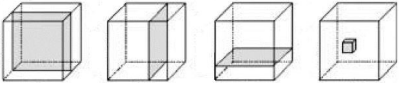
\includegraphics[scale=1]{figures/cube_ops.png}
\caption{Operazioni sui cubi}
\end{figure}
\end{center}

Questi oggetti prendono il nome di misure all’interno dello spazio e possiamo utilizzarli per avere tanti tipi diversi di relazioni. La finalità è quella di fare operazioni sintetiche a livello alto della piramide di Anthony. 


\subsection{Operazioni concettuali}

Consideriamo ora uno spazio a n dimensioni. Le operazioni concettuali che posso effettuare su questo spazio sono: 

\begin{itemize}

\item La prima operazione che possiamo fare è quella di espandere lo spazio del punto prendendo una sfera o ridurre la stessa fino a farla diventare un punto. Se aggreghiamo tutti i fatti attorno ad una certa coordinata, sapremo, riferendoci all’esempio di prima, quanti pezzi sono stati venduti di tutti i prodotti, i pezzi usciti dalla cassa e il prezzo medio. Possiamo aggregare lungo una certa dimensione, non considerando il fatto elementare ma la somma, media o un qualunque operatore di natura statistica. A questo punto espandendo lungo una 
certa dimensione non consideriamo più il fatto elementare, ma il fatto aggregato. Questa 
operazione di espansione si chiama “drill down” (espressione che viene dal mondo del data mining: qui si immagina che il database sia una miniera mentre noi siamo i minatori che scopriamo diamanti corrispondenti alle informazioni). Nello specifico, abbiamo un prisma aggregato e lo spezzettiamo nei sotto cubi finché troviamo il fatto elementare. 

\begin{center}
\begin{figure}[H]
\centering
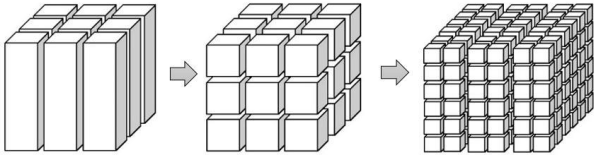
\includegraphics[scale=1]{figures/drill_down.png}
\caption{Operazione di DRILL-DOWN}
\end{figure}
\end{center}

Alternativamente abbiamo l’operazione di “roll up” o di aggregazione (invece di vedere tutti i valori analitici osserviamo il valore sintetico). Queste due sono le stesse operazioni percorse però nelle direzioni opposte. 

\begin{center}
\begin{figure}[H]
\centering
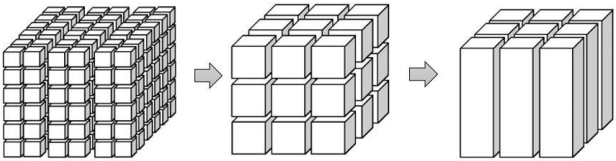
\includegraphics[scale=0.8]{figures/roll_up.png}
\caption{Operazione di ROLL-UP}
\end{figure}
\end{center}

\item La seconda operazione è lo “Slice and dice”, ossia prendiamo un cubo, lo tagliamo a fette e successivamente a dadini (eventualmente quei dadini li dividiamo in sottocubi): un cubo aggregato è tutta l’informazione, invece i dadini sono paragonabili ad una query;

\item La terza operazione è il “Pivot”, in cui invertiamo due assi cartesiani (scambiando la $x$ con la $y$) oppure in uno spazio a n dimensioni ruotiamo il sottospazio. Di solito abbiamo $y=f(x), x$ è la variabile indipendente e $y$ è dipendente. Quindi avremo $x=f^{-1}(y)$. Invertendo gli assi possiamo capire se rappresentare il fenomeno: in questo modo fornisce una relazione di causa effetto e potremmo ricondurci eventualmente ad un pattern ricorrente (lo strumento per effettuare pivot su Microsoft è Excel interfacciabile su Analisys Services, mentre su Pentaho è Mondrian). 

\begin{center}
\begin{figure}[H]
\centering
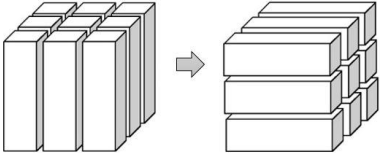
\includegraphics[scale=1]{figures/pivoting.png}
\caption{Operazione di PIVOTING}
\end{figure}
\end{center}

\end{itemize}



\begin{flushright}Giuseppe D'Amuri\\Federico De Luca\\17/11/2016\end{flushright}


\section{Analisi Multidimensionale e Data Warehousing}

In realtà nel multidimensionale si utilizzano molti concetti dei normali DB. Ritroviamo la metodologia tipica di progettazione di un DB, che viene suddivisa in: progettazione a livello concettuale, quella a livello logico e quella a livello fisico. Nei DW si utilizza un'architettura a tre livelli (Three-tier).  

\begin{center}
\begin{figure}[H]
\centering
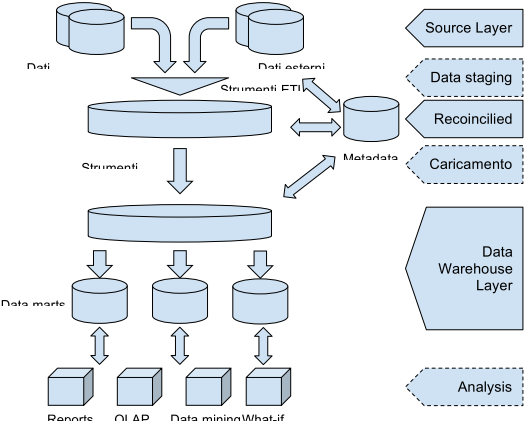
\includegraphics[scale=0.8]{figures/DW_three_tier.png}
\caption{Architettura Three-Tier per i DW}
\end{figure}
\end{center}

In uno scenario classico le diverse organizzazioni o compartimenti dialogano effettivamente tra di loro, ma non hanno le stesse informazioni. Per questo nel mondo reale prima di tutto è necessario spendere nell'eseguire la cosiddetta operazione di Data Integration. Non vi è un mero problema di diversità fisica: il vero problema è che questi dati possono essere sia espressi che interpretati diversamente. Se combinati opportunamente però, questi dati alla fine possono risultare molto esplicativi ed utili, in grado di risolvere molti problemi di ambiguità o mancanza di informazione se visti isolatamente. All'interno di un DB isolato i dati sono tutti consistenti tra di loro. Noi invece abbiamo bisogno di effettuare una collezione di questi pezzi e renderli consistenti anche a valle della combinazione, risultando quindi alla fine sovrapponibili. Nel primo livello dell'architettura, denominato Source Layer abbiamo tutti i dati provenienti da differenti sorgenti, non necessariamente DB, in un unico DB che è chiamato Schema Riconciliato, facente parte del secondo strato dell'architettura denominato Reconcilied Layer. I dati che a monte giungono qui provengono quindi da differenti ambienti, e vengono diversificati in Dati Operazionali e Dati Esterni. I primi provengono tipicamente da DB visti sino ad ora, e concretizzano le operazioni transazionali CRUD. I dati esterni invece possono provenire da varie fonti. Un esempio di informazione interessante che si potrebbe ricavare consultando i Dati Riconciliati è la flessione delle vendite, che oltre a considerare soltanto le vendite di veicoli, questi dati devono essere incrociati magari anche con l'aumento del prezzo del petrolio, oppure con i cambi delle varie valute etc.. Quindi non abbiamo bisogno soltanto di informazioni Operazionali, ma anche di quelle Esterne. Inoltre troviamo qui anche i Metadati che devono essere presi in considerazione; essi servono a contestualizzare i dati che provengono da un certo ambiente. Ad esempio, in concomitanza con i dati sulla vendita, potrebbe essere utile riportare la procedura di ordinazione utilizzata dagli utenti in una determinata vendita. Sostanzialmente sono delle informazioni ausiliarie, di contesto, che però devono essere messe assieme alle precedenti per ottenere un maggiore comprensione del fenomeno. Nel passaggio dallo strato dei Dati Riconciliati al Data Warehouse vero e proprio, che fa parte dell'ultimo strato della Three-tier per i DW, avvengono le cosiddette operazioni ETL (Extraction, Transformation and Loading), ovvero di estrazione, di trasformazione e di caricamento. Nella descrizione di questa fase è bene tenere presente che a valle della procedura di Data Staging, ovvero di raccolta dei dati dalle varie fonti e nell'immissione nello strato dei Dati Riconciliati, i dati non sono puliti e non sono completi a volte. Tipicamente prima di essere immessi nel DW vero e proprio devono essere firmati da un responsabile e devono obbligatoriamente essere verificati. Una volta che i dati sono arrivati quindi, bisogna effettuare delle verifiche di consistenza e di validità/solidità, e solo dopo vengono immessi nel DW. Il DW può contenere tutta la storia della mia azienda. Mentre i Dati Riconciliati risiedono su un DB tipicamente relazionale, quelli nel DW sono immagazzinati in uno schema multidimensionale. Naturalmente la quantità dei dati presenti nel DW è molto più grande! In grandi aziende si scrivono GB di dati solo come LOG, è auspicabile aspettarsi quindi un paio di ordini di grandezza in più per i dati immagazzinati veri e propri. Il DW è quindi un oggetto che deve essere ottimizzato. Si tenga presente che nel multidimensionale non ci sono JOIN, ma sono molto prestanti le operazioni di aggregazione. Per raggiungere comunque delle performance ottimali, bisogna suddividere il DW, che di per sè è un vero e proprio ipercubo di dati, in sottocubi tematici denominati Data Mart. Ognuno rappresenta soltanto una parte dei dati racchiusi nel DW, diversificati per Area Tematica. In genere si progettano direttamente i Data Mart, anche se tecnicamente i dati alla fine devono comunque essere messi insieme. A questo punto abbiamo i quattro mondi più diffusi per effettuare Analisi Dati: abbiamo i Report che sono uno strumento cartaceo dettagliato di analisi. Un esempio potrebbe essere la Dichiarazione dei Redditi od il Bilancio Annuo che le aziende sono tenute a fare. Consistono sostanzialmente nella storicizzazione certificata del DB in un certo giorno. Esistono degli appositi framework, uno dei quali è BIRT (Business Intelligence Report Tool), che è open source e fornisce come output un documento in molti formati disponibili. Anche in Word esiste la possibilità di creare un report e collegarlo ad una o più tabelle del DB. Permette una formattazione più efficiente rispetto ad Access. Ma si tenga presente che questi documenti vanno alla fine stampati. Il mondo della reportistica è quindi un mondo su carta essenzialmente. Vi è una notevole differenza tra dati al computer e dati su carta: vi è tutto un discorso di responsabilità; Poi abbiamo gli strumenti OLAP (Online Analytics Processing), che permettono una navigazione sui vari cubi. Su di essi si può effettuare la ricerca di correlazioni e contemporaneamente navigarli alla stregua di normali pagine web. Sono sostanzialmente delle applicazioni navigazionali; Un altro strumento è il Data Mining, che si compone a sua volte di tecniche di Business Intelligence e Decisions Support Systems tipo il Pattern Recognition, Clustering, Expectation/Maximization (EM), etc. Grazie a questi strumenti oggi con i Big Data si va verso una prospettiva scientifica molto differente. Si possono acquisire i dati di tutto il mondo e capirne il funzionamento semplicemente attuando queste tecniche, ovviamente facendole eseguire da un calcolatore. Si citino anche come importanti tecniche il Pattern Matching ed il Machine Learning; poi abbiamo anche strumenti What-If, che permettono di estrarre un modello matematico rappresentativo del fenomeno, che può simulare ad esempio il funzionamento di un'azienda. \`E in realtà un mondo nato da Excel, tanto è vero che in Excel è possibile fare un'estrapolazione prendendo l'andamento in un intervallo proiettandolo in avanti. Si possono effettuare delle Analisi Variazionali di particolari fenomeni variandone i parametri. Oggi ci sono però degli scenari più complessi oltre al già citato cosiddetto Business Game. Ci possono essere delle reti di Business Game collegati alla previsione di andamenti di differenti aziende andando ad incrociare i vari andamenti, che magari si influenzano reciprocamente. Ma non si simula solo il business in realtà. Questi strumenti sono utilizzati anche nell'ambito dello studio dei Cambiamenti Climatici. Esistono delle tecniche apposite di proiezione di tanti scenari eterogenei con modelli differenti. Tutto questo mondo si appoggia sui DW. 
 
Riguardo l'ETL, abbiamo che l'Estrazione può essere Statica, nella quale i dati vengono accumulati una sola volta, oppure incrementale o dinamica, ove si può scegliere di inserire i dati per l'appunto incrementalmente, per esempio quelli riguardanti l'ultimo mese. Riguardo la PULITURA, una fase preliminare alla trasformazione vera e propria, ma che può essere inglobata in quest'ultima, essa si esplode in eliminazione di dati duplicati: a volte possiamo avere degli interi dataset duplicati; risoluzione dell'inconsistenza dei dati o tra dati diversi. Possiamo andare incontro a situazioni di dati mancanti, che in questa fase devono essere opportunamente gestiti. Per ognuna di queste esistono delle tecniche apposite, tipo algoritmi Minimum Edit Distance o basati sulla distanza di Hamming tra stringhe, tecniche tutte inglobate nella Data Cleaning oppure Data Cleansing. La fase di Trasformazione vera e propria si compone invece delle fasi di Aggiunta Metadati e di Normalizzazione ove si indicizzano opportunamente i vari campi del dato, di Standardizzazione ove si portano i dati secondo convenzioni comuni e successivamente quella di Correzione, ove si correggono eventuali dati sbagliati. Esiste il problema del carico di lavoro: a rigore ogni qualvolta si alimenta il DW bisognerebbe ricalcolare gli indici. Per questo motivo un DW viene alimentato tipicamente ogni due/tre mesi. Si effettuano quindi dei report bimestrali/trimestrali. 

\begin{center}
\begin{figure}[H]
\centering
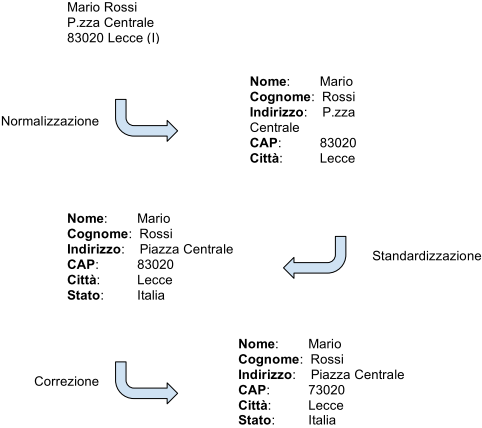
\includegraphics[scale=0.8]{figures/etl.png}
\caption{ETL: Normalizzazione, Standardizzazione e Correzione}
\end{figure}
\end{center}

Un DW è sostanzialmente un ipercubo di dati. Ognuno dei cubetti di cui si compone internamente il cubo rappresenta un Fatto Elementare (dato a granularità minima del DB multidimensionale). Tutti i DB multidimensionali presentano il problema della SPARSIT\`A. Nel tipico scenario Cliente Acquista Prodotto, rappresentato opportunamente nel DW, un negozio potrebbe stare chiuso in una certa data oppure qualche prodotto/parte potrebbe non essere in vendita in un certo negozio. Bisogna gestirla opportunamente. I motori grafici utilizzano lo stesso approccio basato sulle matrici multidimensionali che si utilizzano nei DW. Una serie di fotogrammi non è nient'altro che la giustapposizione temporale di matrici 2D; ancora, la profondità di un oggetto a livello di singolo pixel è gestito dal cosiddetto Z buffer. La profondità viene quindi associata ad un buffer multidimensionale. Un cubetto per noi è semplicemente un fatto che è accaduto o meno. Si utilizzano delle tecniche come il Pattern Matching/Recognition per trovare delle regolarità e classificare alcuni fatti. Si tratta semplicemente di individuare delle strutture geometriche che si ripetono. Tornando al problema della sparsità, se abbiamo tre dimensioni e 1000 elementi ad esempio, si arriva a dover gestire un oggetto dimensionalmente composto da 1000x1000x1000 elementi. Si arriva facilmente a numeri come $100^{25}$ quando si lavora ad esempio con 25 dimensioni da 100 elementi. Ma queste matrici non sono DENSE ma SPARSE! Se abbiamo elementi nulli (non popolati), non li memorizziamo! Vi è tutto un discorso sulla costruzione apposita degli indici per gestire queste situazioni. All'aggiunta di un nuovo fatto quindi, il processore dovrebbe ripercorrere tutto il DB. Si utilizzano quindi tecniche GPGPU per effettuare il parallelismo MIMD massivo ed utilizzare un numero elevato di processori in parallelo per processare questi dati. 

Con le matrici multidimensionali le Query possibili sono essenzialmente di tre tipi: quelle di tipo SLICING, ottenute applicando la tecnica SLICE \& DICE, ove genericamente si estraggono dei piani, dei cubi, delle colonne. Un'altra operazione molto importante è l'AGGREGAZIONE sulla base di Gerarchie Multidimensionali. Ogni tipo si differenzia in singolo prodotto. Vendita per Categoria/Tipo/Prodotto. Tramite tecniche di ROLL-UP e DRILL-DOWN congiuntamente ad operazioni S\&D si naviga attraverso le gerarchie multidimensionali. Un’aggregazione si compone quindi di ROLL-UP e DRILL-DOWN. Si effettuano quindi delle proiezioni, ove si proietta un qualsiasi ipercubo multidimensionale nello schermo 2D. Questa navigazione nella gerarchia multidimensionale è detta Navigazione OLAP. L'operazione di DRILL-DOWN mette in luce eventuali sparsità. Con l'operazione di PIVOTING effettuiamo ricerca di eventuali correlazioni, da non confondersi con le relazioni di causalità (causa-effetto) tra eventi. Una volta trovata un'eventuale correlazione non sappiamo chi è la causa e chi l'effetto!  

Tecniche di Data Mining: sono delle tecniche che permettono di trovare delle regole associative. Ad esempio, l'implicazione vendita delle scarpe $\rightarrow$ vendita delle calze. Si introducono concetti come Supporto, Confidenza. Sulla base di tutte queste tecniche ed operazioni si effettua la cosiddetta MBA (Market Basket Analysis). Le tecniche di clustering sono molto importanti in questo. I dati vengono aggregati in certi gruppi, blocchi, bolle differenti, a seconda della terminologia in uso. Il Data Clustering viene facilitato dall'Analisi Multidimensionale. Il mondo OLTP è quello legato alle transazioni ed al CRUD, mentre il mondo OLAP è quello dei dati analitici, fattibile a diversi livelli. Quando si effettuano delle aggregazioni nel mondo OLAP si parla più propriamente di MOLAP (Multidimensional OLAP); ma anche in SQL abbiamo le operazioni di aggregazione. Quindi l'OLAP è possibile anche su DB operativi, ed in tal caso viene classificato come ROLAP (Relational OLAP). Anche a livello operativo è necessario ricordare la storia dei clienti. Si utilizzano quindi eventuali strumenti DSS di supporto alle vendite. Nella piramide DMO di Anthony troviamo non solo gli strumenti operativi, ma anche decisionali! Ma non solo a carico della direzione c'è bisogno di queste cose, ma anche in piccolo, nello strato transazionale/operativo quindi.  In generale è bene sfruttare le interfacce per effettuare delle Query Proattive. La differenza di Google con Facebook è che su quest'ultimo le cose più importanti ce le dice già lui senza che interagiamo con esso! I compleanni degli amici ad esempio. Si effettuano le interrogazioni più importanti e le si propongono successivamente all'utente. Queste non sono altro che KPI, in piccolo, ed il loro ottenimento rappresenta un esempio di applicazione OLAP a livello di DB relazionale, operativo $\rightarrow$ ROLAP.  

Ciclo di vita DW. Dietro la progettazione di un DW ci sono delle scelte strategiche importanti. Vi sono due approcci: Approccio Top-Down e Bottom-Up. Nel primo vi è un ordine di priorità. Sulla base di quello che il committente vuole, noi proponiamo e via via comunichiamo il costo, scendendo sempre più in dettaglio a partire dal problema. Questi approcci tipicamente sono congiunti ad una Ristrutturazione Aziendale che comporta la scelta di regole drastiche e l'impiego di operazioni onerose. Queste tecniche forniscono i migliori risultati ma portano al dover scontrarsi con dei cambiamenti anche molto duri talvolta. Sono richieste quindi delle persone esperte: non è una questione di tecnologie. Non è solo il risultato a dover essere tecnicamente buono. 

Poi abbiamo l'approccio Bottom-Up. Aproccio che parte da dei DB già fatti bene, dai quali possiamo estrarre degli indicatori (KPI) interessanti. Via via astraiamo dai dettagli di livello più basso per selezionare i vari elementi di cui si comporrà alla fine il DW.  

DATA MART. Si parte da un primo Data Mart, ad esempio quello relativo al settore vendite, che tipicamente è il più prioritario. Dopo un certo tempo avremo il relativo Data Mart definitivo relativo alle vendite, ma nel frattempo possiamo lavorare in parallelo su Data Mart di altri settori.  

Ricordiamo ora le varie fasi che compongono il ciclo a cascata della progettazione: Analisi e Conciliazione delle Sorgenti assieme all'Analisi dei Requisiti, Progettazione concettuale, Raffinamento del carico di lavoro, Progettazione logica, Progettazione dell'Alimentazione e progettazione fisica (DB). Si effettuano delle interviste al personale che dirige l'azienda, adottando un modello a Piramide o ad'Imbuto. L'obiettivo è comunque sempre lo stesso. Approccio a piramide (Bottom-Up) ed approccio ad imbuto (Top-Down). Così come nei DB utilizziamo dei Design Pattern, nel mondo DW abbiamo già delle soluzioni a problemi standard incontrati di frequente. Nei DW quindi abbiamo dei fatti significativi che esso deve contenere. Ma da quale DB vengono queste informazioni? Ad esempio potrebbe esserci un Data Mart apposito per il CRM (Customer Relationship Management) ove tipicamente si esercita la gestione dei reclami ad esempio. Bisogna scavare e trovare i settori dell'azienda all'interno dei quali queste informazioni sono rilevanti. \`E utile a tal proposito una tabella a singola entrata con due colonne: {Data Mart, Fatti Rilevanti}. In funzione del tipo dell'azienda si imposta un certo tipo di progettazione.  

Ora subentriamo in una specifica parte delle tecniche di progettazione. Nei DB ci sono gli ER. Qui abbiamo i DFM (Dimensional Fact Model), comunque collegati ai DB ma sono visti da un punto di vista differente. I DW si possono progettare a livello logico con gli schemi a stella. Modello Concettuale, Fisico e Logico sono sempre presenti. I Fact Model sono a livello concettuale. Essi servono per trasformare i fatti aziendali in tabelle multidimensionali. Ogni fatto ha un nome. In Cliente Acquista Prodotto abbiamo il fatto Vendita. La vendita come relazione è al centro. In una particolare configurazione DFM, la vendita potrebbe dimensionalmente essere associata ad una Data, ad un Prodotto e ad un Negozio. Questa potrebbe essere la reificazione o proprio la vera e propria relazione. In VENDITA ci mettiamo le misure. il prezzo unitario è una caratteristica del prodotto, ma può essere riportato anche in VENDITA. Esiste anche un altro campo al quale in realtà non siamo abituati. Si chiama Numero Clienti. Valore unitario che si mette per agevolare le operazioni di conteggio/aggregazione. Molto spesso ci sono dei fatti che non hanno alcuna misura al loro interno. Ma il fatto che succeda e quando succeda è già significativo. Non possiamo fare una valutazione quantitativa! Un fatto esprime un'associazione molti-a-molti tra le varie dimensioni. Invece le dimensioni nel nostro caso sono {{data}, {prodotto}, {negozio}}. Immediatamente dopo aver definito il fatto, definiremo le Gerarchie Multidimensionali. Prodotto $\rightarrow$ Marca $\rightarrow$ Città. Questi successivi raggruppamenti definiscono delle gerarchie in una stessa dimensione. Difatti potremmo esser interessati alle vendite di un certo prodotto di una certa zona. Non mi basta sapere la marca, ma anche ad esempio se vi sono dei prodotti a Km/0. Si parla proprio di tendine nella navigazione di queste gerarchie. Navigandoci dentro per l'appunto, si compiono nient'altro che le già citate operazioni di Aggregazione che si compongono di ROLL-UP e DRILL-DOWN. Prodotto $\rightarrow$ Tipo $\rightarrow$ Categoria. Il Negozio può ad esempio esser suddiviso per Responsabile delle Vendite. Le performance è perfettamente auspicabile che si suddividano in base al responsabile oppure al distretto delle vendite. Ci possono essere delle aggregazioni non dimensionali bensì alternative. Un'altra aggregazione molto importante è quella sulle Date delle vendite. Le Date si compongono di vari campi elementari YYYY/MM/DD/H/M/S, i quali nel loro insieme formano la data. Potremmo avere dei raggruppamenti successivi per giorno o per settimane. Le settimane sono abbastanza importanti. In alcuni casi potrebbe essere molto significativo vedere gli eventi di interesse in base alla settimana. Abbiamo quindi Data $\rightarrow$ Settimana $\rightarrow$ Mese $\rightarrow$ Giorni di Vendita oppure Giorni Lavorativi. Queste ultime due sono delle Associazioni Ortogonali tra di loro. Sono distinte, diverse. Una stessa data può essere di vacanza o lavorativa per differenti negozi. Ogni nodo prende il nome di Attributo Dimensionale. Le interrogazioni sono alla fine dei percorsi che tracciamo nel grafico dei fatti. Abbiamo una n-upla di attributi dimensionali. Queste sono le cosiddette Query MDX (Multidimensional Expressions). Non sono nient'altro che delle n-uple o tuple di attributi dimensionali. Ma come funziona l'RDB che sta dietro? Partendo da degli RDB si mettono insieme e si arriva a definire il cosiddetto Database Riconciliato. Qui tutte le gerarchie sono esplose in successive relazioni (1-n). Avremo ad esempio i tipi di entità DATA, che può essere di vacanza o lavorativa ed appartenere via via agli altri vari attributi dimensionali omogenei nella stessa entità. Nel database dovremmo inoltre tenere conto di dettagli relativi alla Località. Infatti una certa data può essere di vacanza per un certo stato ed essere invece lavorativa per un altro. Questi vengono detti attributi CROSS-DIMENSIONALI. Esattamente come ci si aspetta in un albero gerarchico, sono tutte relazioni (1-n). Le ridondanze non sono in questo caso molto preoccupanti. Tutti questi elementi sono candidati a divenire gerarchie multidimensionali. Qui noi vogliamo ottimizzare le query, le interrogazioni. Qualche ridondanza ci può ovviamente stare, e talvolta sarà proprio necessaria.  

\`E importante comprendere la differenza tra DB operativi e quelli analitici. Alla fine le attività commerciali si strutturano sempre in vendite di prodotti e di servizi, ad esempio. Tipicamente esistono delle gerarchie standard abbastanza ricorrenti: le Gerarchie Spaziali, le Gerarchie Temporali. Inoltre avremo poi le Gerarchie Specifiche del problema. Sono alla fine dei concetti abbastanza logici ed intuitivi.  

Come si fa invece a capire quali sono i fatti del mio RDB? Possiamo utilizzare un approccio Top-Down o Bottom-Up. Tipicamente i Fatti Significativi sono quelli che accadono più frequentemente. Il fatto cruciale sarà quello più frequente ed importante in assoluto: la VENDITA nel nostro caso. Non sarà DATA ad esempio, in quanto il calendario aziendale è già stabilito ad inizio anno. Non sarà PRODOTTO, in quanto il catalogo dei prodotti è già stabilito dall'azienda all'inizio dell'anno. Ci possono essere delle variazioni, ma non cambia nulla. La VENDITA è il fatto significativo, tra l'altro anche perché si aggiungono sempre, in base al principio di NO-DELETE. In tutto quindi quanti fatti ci sono? Due o tre sul cliente, in quanto le variazioni sul cliente sono locali e registrate nella relativa entità stessa. Un paio di fatti sul PRODOTTO. Tutti gli altri eventi sono a bassissime frequenze rispetto alle vendite. Distinguiamo quindi gli Eventi Primari da quelli Secondari. Esistono anche gli Attributi Opzionali, presenti solo nel qual caso ad esempio un Prodotto appartenga ad una determinata categoria (es. attributo dieta solo su prodotti di categoria alimentare). Possono anche esserci degli Attributi Descrittivi, i quali non servono propriamente a fare le operazioni di Aggregazione, quanto invece per avere informazioni più dettagliate su una certa dimensione di un fatto all'interno della sua relativa gerarchia dimensionale. 

\begin{center}
\begin{figure}[H]
\centering
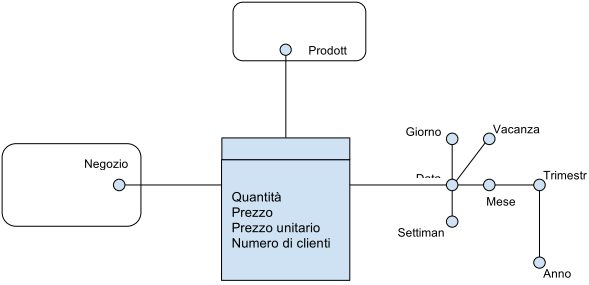
\includegraphics[scale=1]{figures/fact_model.png}
\caption{Dimensional Fact Model: DFM}
\end{figure}
\end{center}



\begin{flushright}Marco Chiarelli\\Paolo Panarese\\23/11/2016\end{flushright}


\section{COSTRUTTI AVANZATI DEL DFM}

\begin{itemize}

\item{\underline{\textbf{ATTRIBUTI CROSS-DIMENSIONALI}}}:

Sono attributi che dipendono da più dimensioni (appartenenti a diverse gerarchie). Un classico esempio è l’IVA: essa varia da stato a stato, ma anche in base alla categoria dei prodotti (i beni di prima necessità presentano un’aliquota IVA inferiore a quella dei beni di lusso).  
 
\begin{center}
\begin{figure}[H]
\centering
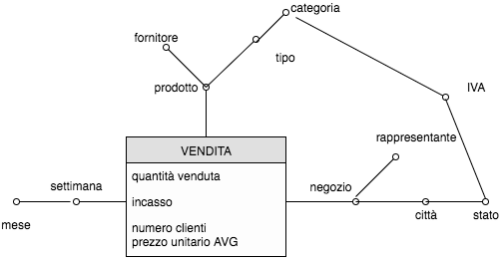
\includegraphics[scale=1]{figures/cda.png}
\caption{Attributi Cross-Dimensionali}
\end{figure}
\end{center}

\item{\underline{\textbf{ARCO MULTIPLO}}}:

\begin{center}
\begin{figure}[H]
\centering
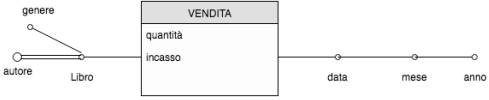
\includegraphics[scale=1]{figures/ma.png}
\caption{Arco Multiplo}
\end{figure}
\end{center}

Generalmente le associazioni fra attributi dimensionali sono 1:N. L’arco multiplo consente di rappresentare, invece, un’associazione N:M.  In questo esempio si aggregano le vendite di libri in base agli autori. Un autore scrive più libri, ma un libro può anche essere scritto da più autori. Per questo motivo è necessario utilizzare un arco multiplo. Per dare maggiore consistenza alle aggregazioni tramite archi multipli, si devono attribuire dei “\textbf{pesi}” (ad esempio, un autore scrive un libro per il 90\% e l’altro per il 10\%; i pesi consentiranno di gestire le diverse percentuali degli incassi da attribuire ai due autori). 

\item{\underline{\textbf{ADDITIVIT\`A}}}:

Al fine di aggregare i fatti, è necessario definire gli operatori che lavoreranno sui valori delle misure. Queste ultime possono essere di tre tipi:

\begin{itemize}

\item{MISURE DI FLUSSO}: riferite ad un periodo di tempo, ad es. flussi di merce, di denaro, di cassa, il numero di prodotti venduti in un giorno, l’incasso                                              mensile, il numero di nati in un anno;
\item{MISURE DI LIVELLO}: valutate in un dato istante di tempo (numero di pezzi in                                               magazzino);
\item{MISURE UNITARIE}: valutate in istanti di tempo, ma in termini relativi (prezzo                                             unitario di un prodotto, percentuale di sconto).   

\end{itemize}

\textit{Esempio}

Consideriamo una misura di livello: supponiamo che la mia azienda abbia in cassa 1000 euro nella sede di Lecce e 1000 euro in quella di Brindisi. La cassa, in totale, ha 2000 euro (posso sommare su gerarchie spaziali). Supponiamo, ora, che nella cassa di Lecce, alla fine della giornata di ieri, ci fossero 1000 euro, e che oggi ce ne siano 1000. In questo caso non posso sommare e affermare di avere in cassa 2000 euro! (la somma su gerarchie temporali non è consentita).  

La tabella seguente indica quali operazioni sono consentite relativamente ai tipi di gerarchie: 

\begin{center}
\begin{figure}[H]
\centering
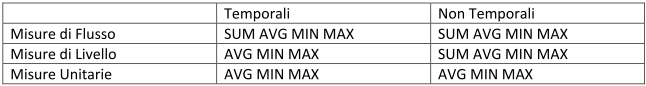
\includegraphics[scale=0.8]{figures/tabella_misure.png}
\caption{Tabella Tipi di Misure}
\end{figure}
\end{center}

Una misura, dunque, si dice \textbf{ADDITIVA} su una dimensione se i suoi valori si possono aggregare lungo la corrispondente gerarchia con l’operatore di somma, altrimenti è detta \textbf{NON ADDITIVA}.

\begin{center}
\begin{figure}[H]
\centering
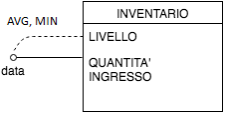
\includegraphics[scale=1]{figures/inventario.png}
\caption{Inventario FACT}
\end{figure}
\end{center}

L’arco tratteggiato indica la “non additività”, e AVG e MIN indicano che l’aggregazione è consentita soltanto tramite gli operatori di media e minimo.   

\item{\underline{\textbf{SCHEMI DI FATTO VUOTI}}}:

\begin{center}
\begin{figure}[H]
\centering
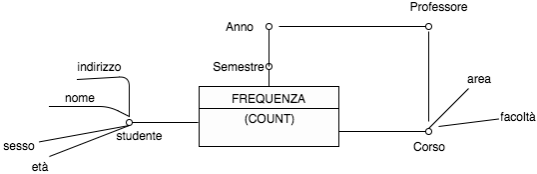
\includegraphics[scale=1]{figures/efs.png}
\caption{Empty FACT Schema}
\end{figure}
\end{center}

Sono fatti che non hanno misure. Servono principalmente a registrare il verificarsi di un evento, ad esempio la frequenza con cui uno studente segue un corso. Nel fatto Frequenza non troviamo misure, ma solo un contatore. 

\end{itemize}


\subsection{ESEMPIO DELLE VENDITE (DA E/R)}

Al livello dei dati riconciliati, nel modello ER si devono esplicitare le gerarchie dimensionali e i fatti di business.

\begin{center}
\begin{figure}[H]
\centering
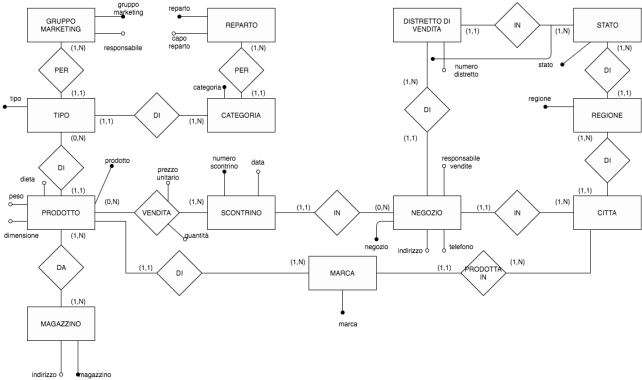
\includegraphics[scale=0.8]{figures/riconciliato_vendite.png}
\caption{DB Riconciliato: VENDITE}
\end{figure}
\end{center}

I pallini scuri indicano che un particolare attributo è chiave primaria.

\subsection{Passaggio dall’ER riconciliato al DFM: l’ALBERO DEGLI ATTRIBUTI}

Il passaggio dal modello ER dei dati riconciliati al DFM avviene tramite un algoritmo di mapping, che mira a costruire il cosiddetto “\textbf{albero degli attributi}”, in cui la radice è il fatto, mentre ogni entità connessa al fatto è un nodo dell’albero. 

\begin{center}
\begin{figure}[H]
\centering
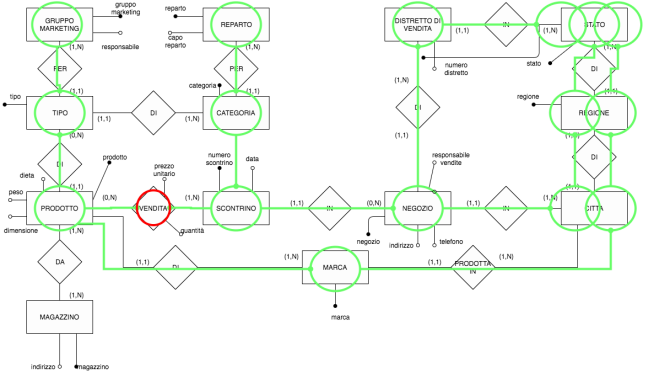
\includegraphics[scale=0.8]{figures/pre_attributes_tree.png}
\caption{Individuazione Radice e Nodi su un DB Riconciliato}
\end{figure}
\end{center}

Individuati (figura sopra) la radice e gli altri nodi, si costruisce l’albero degli attributi:

\begin{center}
\begin{figure}[H]
\centering
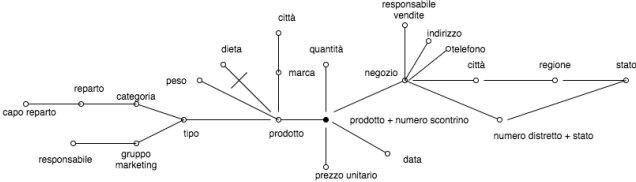
\includegraphics[scale=0.8]{figures/attributes_tree.png}
\caption{Albero degli Attributi}
\end{figure}
\end{center}

Sull’albero degli attributi si possono effettuare due operazioni:  

\begin{itemize}

\item{POTATURA}: eliminazione di un nodo;
\item{INNESTO}: elimino un nodo e collego i suoi figli direttamente al padre del nodo potato.

\end{itemize}


\subsection{CARICO DI LAVORO}

È un elemento importante da tenere in conto nella progettazione fisica del DW. È necessario stimare quanto incide l’inserimento dei nuovi dati e il ricalcolo degli indici sulle prestazioni del sistema. 


\subsection{PROGETTAZIONE LOGICA}

\begin{center}\underline{\textbf{SCHEMA A STELLA}}:\end{center}

\begin{center}
\begin{figure}[H]
\centering
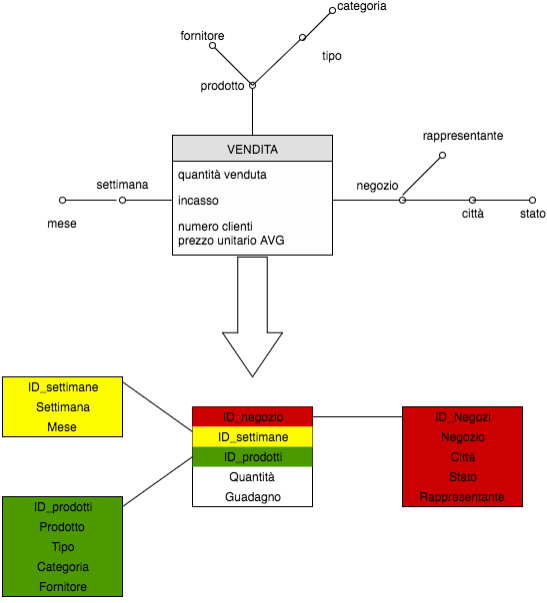
\includegraphics[scale=0.8]{figures/star_schema.png}
\caption{Passaggio da DFM a Star Schema}
\end{figure}
\end{center}

Lo schema a stella è composto da: 

\begin{itemize}

\item{TABELLE DELLE DIMENSIONI}: una gerarchia dimensionale viene “compressa” in un’unica tabella. La chiave primaria della tabella è data dalla   dimensione, mentre gli altri attributi sono costituiti dagli attributi dimensionali;
\item{TABELLE DEI FATTI}: una tabella relativa a un fatto importa (come chiavi esterne) le chiavi di tutte le tabelle delle dimensioni, che insieme diventano chiave primaria       della tabella del fatto.  

\end{itemize}



\begin{flushright}Marco Mameli\\Marco D'Amato\\24/11/2016\end{flushright}


\section{LE TABELLE PIVOT DI EXCEL PER IL DATA WAREHOUSE}

Consideriamo la seguente relazione quaternaria:

\begin{center}
\begin{figure}[H]
\centering
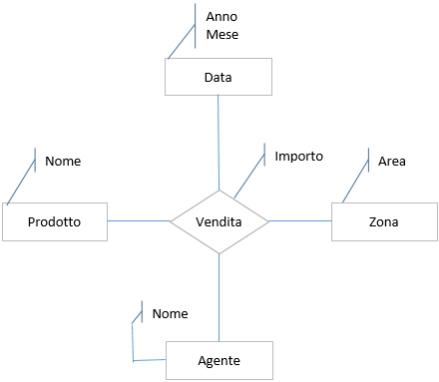
\includegraphics[scale=1]{figures/quat.png}
\caption{Relazione quaternaria VENDITA}
\end{figure}
\end{center}

Da tale diagramma concettuale il fatto più intuitivo e più frequente che si può estrarre è la VENDITA, che in realtà non è altro che la relazione tra le quattro entità. Quindi analizziamo le vendite in base al PRODOTTO, DATA, AGENTE e ZONA:

\begin{center}
\begin{figure}[H]
\centering
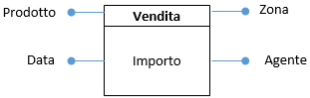
\includegraphics[scale=1]{figures/vendita2.png}
\caption{Vendita FACT}
\end{figure}
\end{center}

La gerarchia temporale completa è:

\begin{center}
\begin{figure}[H]
\centering
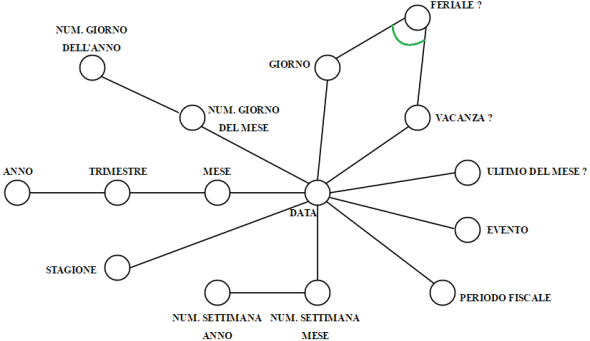
\includegraphics[scale=0.8]{figures/time_hierarchy.png}
\caption{Gerarchia Temporale completa}
\end{figure}
\end{center}

In questo schema vengono indicate con “?” le variabili di tipo booleano. Dato il diagramma ER di partenza e supponendo che tutte le entità abbiano una chiave primaria, immaginiamo di voler fare una query che restituisca una tabella fatta in questo modo:

\begin{center}
\begin{figure}[H]
\centering
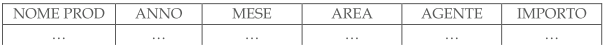
\includegraphics[scale=0.8]{figures/query_res.png}
\caption{Risultato tabellare di una Query}
\end{figure}
\end{center}

Se si volessero conoscere i prodotti inseriti, in Excel si può selezionare la colonna prodotti e una volta ricopiata, tramite la funzione “rimuovi duplicati” in “dati” che si trova sul pannello, si può vedere quali sono i vari prodotti distinti. La stessa cosa si può fare con le altre misure. Si osserva in questo caso che si hanno tre tipi di prodotto, due anni, diversi mesi, due agenti e due aree.  

Andiamo a creare ora la tabella PIVOT, uno strumento analitico di reporting necessario alla creazione di tabelle riassuntive. Uno dei fini principali di queste tabelle è l'organizzazione di dati complessi tramite una scelta opportuna dei campi e degli elementi che devono comporla. 
    
In Excel si seleziona l’intera tabella dei dati di partenza e si inserisce la tabella pivot andando in “inserisci” $\rightarrow$ “tabella pivot”. Viene creato un nuovo foglio di lavoro in cui è possibile creare tali tabelle riassuntive andando ad agire sui campi della tabella pivot alla destra del foglio.  

\begin{center}
\begin{figure}[H]
\centering
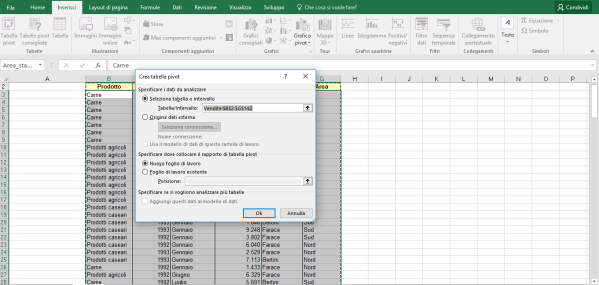
\includegraphics[scale=0.8]{figures/excel_pivot.png}
\caption{Microsoft Excel - Funzione tabella Pivot}
\end{figure}
\end{center}

Ad esempio, se si vogliono analizzare le vendite, si trascina il campo “vendite” nell’area “VALORI”, si può anche decidere il tipo di calcolo da utilizzare, come la somma, il conteggio, la media ecc. cliccando su “impostazioni campo valore”. Se si vuole la vendita dei prodotti distinta per anno, il campo “anno” lo si inserisce nell’area “COLONNE”. Ancora, continuando, si può aggiungere il campo “agente” in “COLONNE” in modo da avere una distinzione per agente in ogni anno.   

Si può contemporaneamente calcolare la somma, il conteggio delle vendite ecc. semplicemente andando a inserire più volte il campo “vendite” in “VALORI” e selezionando le “impostazioni campo valore” opportune. Oppure, come si procede solitamente, si raggruppano più campi sulle “RIGHE”, in questo caso si può raggruppare “anno” e  “mese”:   

\begin{center}
\begin{figure}[H]
\centering
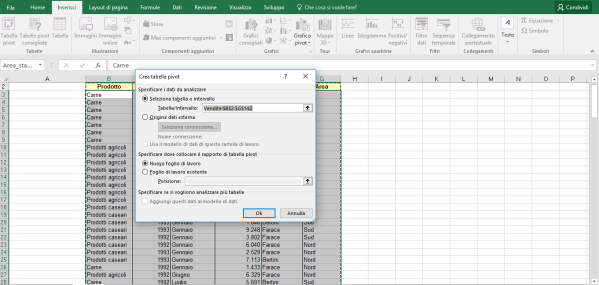
\includegraphics[scale=0.8]{figures/excel_pivot.png}
\caption{Microsoft Excel - Funzioni di Conteggio Somma - Tabella Pivot}
\end{figure}
\end{center}

\textbf{\textit{OSS}}: In questo caso si è riscontrato un problema di data cleaning, nella tabella pivot compare due volte il mese di gennaio perché è stato riportato in maniera errata all’interno del sistema. Bisogna quindi effettuare tutte le operazioni di pulizia opportune durante la fase di ETL (Extract, Transform, Load). Abbiamo corretto il valore errato della tabella di partenza (cella D26) e aggiornato la tabella pivot: “analizza” $\rightarrow$ “aggiorna”.   

\subsection{QUERY} 

\begin{itemize}

\item Incremento percentuale delle vendite (importo) dal 1992 al 1993. COLONNE: Prodotto 

\begin{itemize}
\item{RIGHE}: Anno;
\item{VALORI}: Vendite (somma).
\end{itemize}

\begin{center}
\begin{figure}[H]
\centering
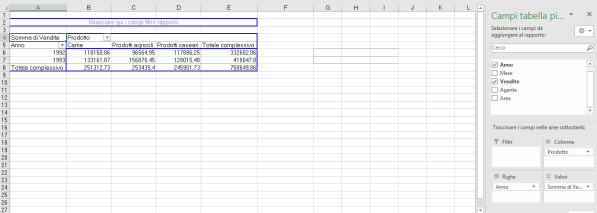
\includegraphics[scale=0.8]{figures/perc_increment.png}
\caption{Microsoft Excel - QUERY Incremento percentuale Vendite}
\end{figure}
\end{center}

Per ottenere il valore in percentuale delle vendite in quel periodo si effettua prima la differenza tra il totale complessivo del '93 e del ’92, il risultato lo si divide per il totale complessivo del ’92 e lo si moltiplica per 100.  

Per migliorare la precisione del risultato, nella sezione “numeri” in “home” si può andare a incrementare o decrementare le cifre decimali.  

\begin{center}
\begin{figure}[H]
\centering
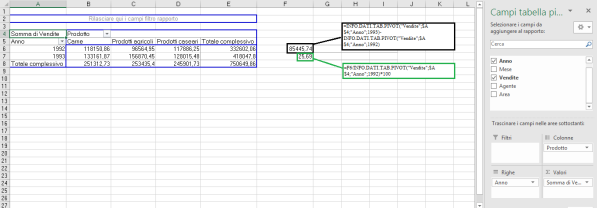
\includegraphics[scale=0.8]{figures/perc_increment_enhanced.png}
\caption{Microsoft Excel - Miglioramento precisione QUERY Incremento percentuale Vendite}
\end{figure}
\end{center}

\item I due mesi in cui si è venduto maggiormente nel ’92;
\item I due mesi in cui si è venduto maggiormente nel ’93.  

RIGHE: Anno, Mese
VALORI: Vendite (somma)  
Per verificare i 2 mesi in cui si è venduto di più si selezionano le colonne mese e totale, le si ricopiano e tramite la funzione “ordinamento personalizzato” in “ordina e filtra” si andrà ad ordinare in modo crescente o decrescente (in questo caso crescente) in base ai totali. La stessa cosa la si fa con l’anno ’93. Si nota che nel ’92 i mesi in cui si è venduto di più sono luglio e maggio, nel ’93 gennaio e maggio.   

\begin{center}
\begin{figure}[H]
\centering
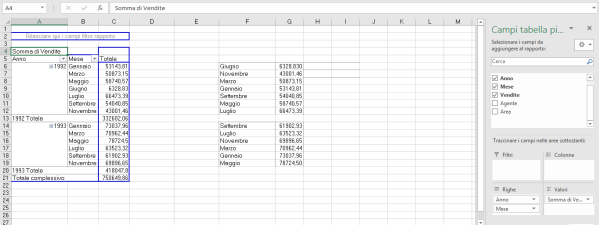
\includegraphics[scale=0.8]{figures/best_months.png}
\caption{Microsoft Excel - QUERY Migliori mesi di Vendita nel '92-'93}
\end{figure}
\end{center}

\item L’area in cui si è venduto maggiormente nel ’92;
\item L’area in cui si è venduto maggiormente nel ’93.  

\begin{itemize}
\item{RIGHE}: Anno, Area;
\item{VALORI}: Vendite (somma).
\end{itemize}

In entrambi gli anni l’area in cui si è venduto di più è il NORD;  

\item L’agente che ha venduto di più nell’area SUD nel ’93.

\begin{itemize}
\item{FILTRI}: Area, Anno;
\item{COLONNE}: Agente;
\item{VALORI}: Vendite (somma).
\end{itemize}

In questo modo si può filtrare l’area e l’anno selezionando quelli richiesti. Per essere sicuri di quale sia il maggiore del valore totale si può utilizzare la funzione MAX tra i valori ottenuti, o andare ad ordinarli come visto in precedenza, in quanto i valori che si ottengono possono essere numerosi (e non 2 come in questo caso).  

\begin{center}
\begin{figure}[H]
\centering
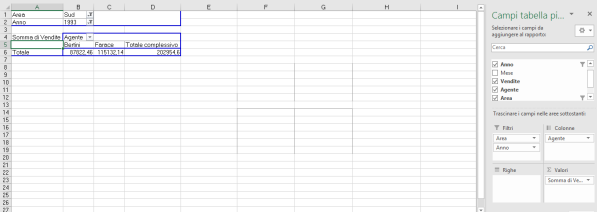
\includegraphics[scale=0.8]{figures/excel_pivotfilters.png}
\caption{Microsoft Excel - Filtri PIVOT}
\end{figure}
\end{center}

L’agente che ha venduto di più è Farace;

\item Il prodotto venduto maggiormente nel ‘92:

\begin{itemize}
\item{FILTRI}: Anno;
\item{COLONNE}: Prodotto;
\item{VALORI}: Vendite (conteggio).
\end{itemize}

\begin{center}
\begin{figure}[H]
\centering
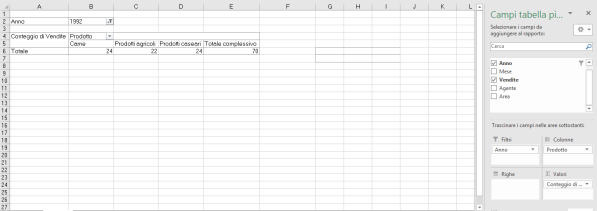
\includegraphics[scale=0.8]{figures/best_product.png}
\caption{Microsoft Excel - QUERY Prodotto venduto maggiormente del '92}
\end{figure}
\end{center}

Selezionato l’anno ’92, i prodotti che risultano più venduti sono la carne e prodotti caseari;

\item Il prodotto che ha fatto incassare di più nel ’92:

\begin{itemize}
\item{FILTRI}: Anno;
\item{COLONNE}: Prodotto;
\item{VALORI}: Vendite (somma).
\end{itemize}

\begin{center}
\begin{figure}[H]
\centering
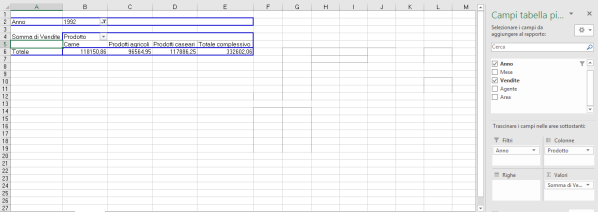
\includegraphics[scale=0.8]{figures/best_pricesum_product.png}
\caption{Microsoft Excel - QUERY Prodotto migliore dal punto di vista degli incassi del '92}
\end{figure}
\end{center}

Selezionato l’anno ’92, il prodotto che ha fatto incassare di più è la carne. Per essere sicuri di quale sia valore maggiore del totale si procede come nella query 6;

\item Prodotto venduto meno nel ’92 nell’area NORD:

\begin{itemize}
\item{FILTRI}: Anno, Area;
\item{COLONNE}: Prodotto;
\item{VALORI}: Vendite (conteggio).
\end{itemize}

\begin{center}
\begin{figure}[H]
\centering
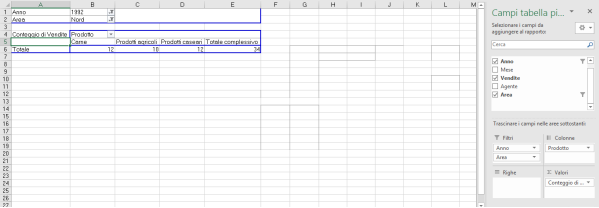
\includegraphics[scale=0.8]{figures/worst_product.png}
\caption{Microsoft Excel - QUERY Prodotto meno venduto nel '92 nell'area NORD}
\end{figure}
\end{center}

Selezionato l’anno e l’area richiesti, il prodotto che ha fatto incassare meno è “prodotti agricoli”. Anche in questo caso per essere sicuri di quale sia il minimo si può andare ad utilizzare le funzioni messe a disposizione da Excel (come la fx MIN o andando ad ordinare ecc.);

\end{itemize}

Immaginiamo ora di avere il seguente scenario, relativo ad un call center: 

\begin{center}
\begin{figure}[H]
\centering
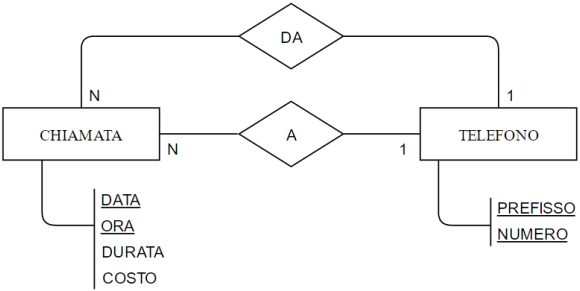
\includegraphics[scale=1]{figures/call_center.png}
\caption{Call Center - ER Scenario}
\end{figure}
\end{center}

\begin{center}
\begin{figure}[H]
\centering
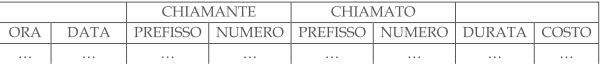
\includegraphics[scale=1]{figures/chiamante_chiamato_table.png}
\caption{Tabella per le query del precedente scenario}
\end{figure}
\end{center}

Il DFM associato è: 

\begin{center}
\begin{figure}[H]
\centering
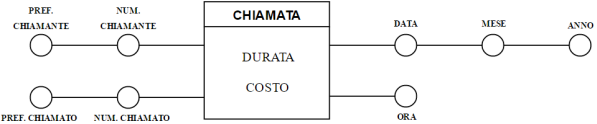
\includegraphics[scale=1]{figures/chiamata.png}
\caption{Chiamata FACT}
\end{figure}
\end{center}

Tale modello però risulta ridondante, cioè porzioni intere di gerarchie risultano duplicate come in questo caso. Utilizzando le gerarchie condivise si ottiene uno schema del genere:

\begin{center}
\begin{figure}[H]
\centering
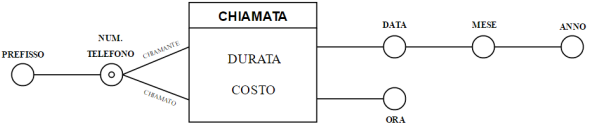
\includegraphics[scale=1]{figures/enhanced_chiamata.png}
\caption{Chiamata FACT - DFM migliorato}
\end{figure}
\end{center}

QUERY:

\begin{itemize}
\item Numero di chiamate senza risposta nel mese di maggio 2016;
\item Il prefisso con le telefonate più lunghe;
\item Il mese del 2016 in cui sono state effettuate più chiamate. 
\end{itemize}



\begin{flushright}Andrea Cuna\\Giuseppe Levantaci\\24/11/2016\end{flushright}


\section{PROGETTAZIONE LOGICA}


\subsection{Indicatori}

Come abbiamo visto nelle lezioni precedenti, un passaggio importante per la creazione di un Data Warehouse è la revisione dei database con la creazione di date e gerarchie di aggregazione; le gerarchie di aggregazione possono essere di tipo temporale, spaziale oppure relative ad un dominio specifico. I Data Warehouse sono aggregazioni di dati multidimensionali in cui, a differenza dei normali database CRUD, sono presenti le operazioni di creazione e modifica, ma non di cancellazione. Perseguono quindi obiettivi diversi. Il modello concettuale di un Data Warehouse è il fact model: un fatto è qualcosa che avviene nel database o nell’azienda; nel primo caso si esegue un approccio di tipo bottom-up, nel secondo di tipo top-down. Si noti come nell’aggregazione dimensionale sia necessario tenere a mente la presenza di un lead time, ovvero il tempo di attraversamento intermedio tra l’attivazione di un processo causato da un evento e la sua conclusione, ad opera di un altro evento.  Uno degli obiettivi di chi crea i database è l’estrazione di indicatori relativi ai tre tipi di risorse (Umane, Materiali, Immateriali). Ad esempio, nel caso di un’università, tali indicatori possono essere: 

\begin{itemize}

\item{Risorse Umane}: livelli di cassa, flusso in uscita (costo risorse umane), numero medio di esami al mese per professore;
\item{Risorse Materiali}: valore fabbricati, costi studenti, valore strumentazione;
\item{Risorse Immateriali}: brevetti, società affiliate.  

\end{itemize}

Schema a stella: È qui riportato lo schema a stella del fatto Acquisto per una catena di supermercati: 

\begin{center}
\begin{figure}[H]
\centering
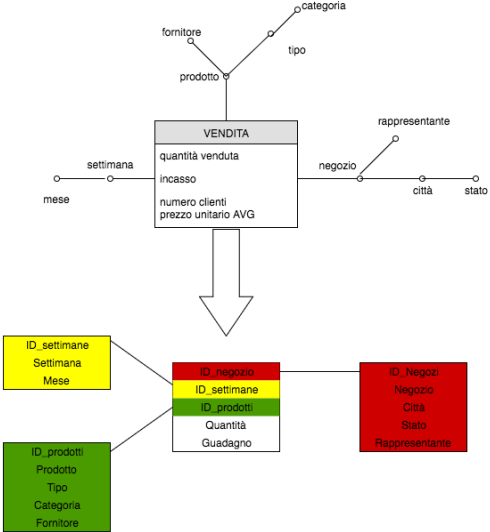
\includegraphics[scale=1]{figures/supermarket_starschema.png}
\caption{Star Schema del FACT Vendita}
\end{figure}
\end{center}

Vengono raccolti tutti i dati di tutti i negozi di un’azienda e così via, aggiungendo successivamente gli ID. La data è vista come un attributo: viene quindi “tirata fuori” e inserita nella gerarchia dimensionale. È importante osservare le dimensioni approssimative delle tabelle. Nel caso della Fact Table, considerando 1000 - 10000 scontrini al giorno saranno presenti circa $10^8$ – $10^9$ righe. La tabella prodotti invece, conterrà 1000 – 10000 righe che non crescono nel tempo: il catalogo dei prodotti resta circa costante. È presente quindi una differenza tra tabelle, suddivise in:

\begin{itemize}

\item{Fact Table}: tabelle grandi e in rapida crescita;
\item{Dimension Table}: gerarchie relativamente piccole e statiche.
\end{itemize}

Si noti la differenza con il modello Entità – Relazioni, in cui le tabelle vengono trattate tutte allo stesso modo. 

\subsection{Motore Data Warehouse}

Le tabelle le cui dimensioni variano poco nel tempo vengono create una sola volta, ad esempio quelle relative a dimensioni spaziali, dimensioni temporali, catalogo prodotti. La Fact Table, invece, è continuamente alimentata. A tal proposito si utilizza un sistema software come “Spoon”: questo è un tool grafico per rappresentare le trasformazioni sui pacchetti; questi vengono poi ripuliti sulla base della provenienza (Excel, Access, MySQL...) e infine inseriti. Infine un sistema come “Mondrian” crea gli indici effettuando i calcoli necessari. 
  
\subsection{SnowFlake Schema}

Le Dimension Table sono completamente denormalizzate: è sufficiente una join per recuperare tutti i dai relativi a una dimensione. Tuttavia la denormalizzazione introduce una parte ridondante nei dati e devono quindi essere normalizzate; se sono presenti troppe join il sistema diventa complesso e difficile da gestire. Esiste la possibilità che esistano più fatti: nel caso di una università, essi possono essere gli esami, o ad esempio i voti degli assignment settimanali. Vengono quindi normalizzate anche altre tabelle, creando sottodimensioni ortogonali tra loro (e quindi indipendenti).  

\begin{center}
\begin{figure}[H]
\centering
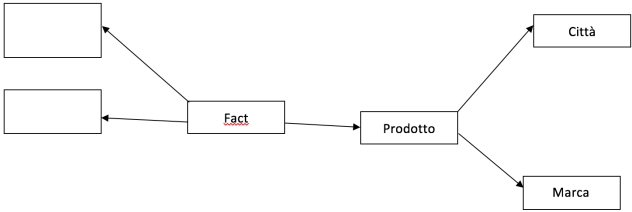
\includegraphics[scale=0.8]{figures/fact_prodotto.png}
\end{figure}
\end{center}

Ora la Fact Table punta ad una serie di dimensioni a loro volta strutturate con pezzi di gerarchie dimensionali. Lo SnowFlake schema può essere quindi visto come uno Star Schema ripetuto a più livelli. Per quanto riguarda le query, non ci sono differenze sostanziali anche se, a causa degli indici diversi, da un punto di vista fisico sono realizzate in maniera diversa. Si pensi ad una gerarchia condivisa con due fatti principali: ORDINE e SPEDIZIONE. Il primo di questi è aggregato in base a Magazzino ed Ordine: quest’ultimi possono essere raggruppati in base alla sottogerarchia spaziale Città (gerarchia di secondo livello).  

Albero degli attributi: si tratta di diverse radici in corrispondenza di determinati fatti; sono usati per la creazione del modello concettuale.  

Riconciliato: vengono riallineati i database relativi ai settori principali dell’azienda (ad esempio Marketing e Vendite).  

L’ultima fase della progettazione di un Data Warehouse consiste nella progettazione del carico del lavoro. Infine i manager navigano gli ipercubi per ottenere i key performance indicator.  



\begin{flushright}Ippazio Alessio\\Simone Dongiovanni\\01/12/2016\end{flushright}